\documentclass{beamer}
\usepackage{graphicx}
\usetheme{default}
\usecolortheme{beaver}
\let\oldAA\AA
\let\oldaa\aa
\def\AA{\^ A}
\def\aa{\^ a}
\def\myqq@{'}
\catcode`\'=13
\def'#1{\ifmmode {}^\prime #1%
         \else\ifx#1a\u{a}%
         \else\ifx#1i\^{\i}%
         \else\ifx#1s\c{s}%
         \else\ifx#1t\c{t}%
         \else\ifx#1A\u{A}%
         \else\ifx#1I\^{I}%
         \else\ifx#1S\c{S}%
         \else\ifx#1T\c{T}%
         \else\ifx#1"\myqq@%
               \fi\fi\fi\fi\fi\fi\fi\fi\fi%
         \fi}

\usepackage{listings}         
\lstset{breakatwhitespace,
tabsize=3,
language=Java,
columns=fullflexible,
keepspaces,
breaklines,
tabsize=3, 
showstringspaces=false,
extendedchars=true}
\newcommand{\HRule}{\rule{\linewidth}{0.5mm}}


\title[]{Corectarea automat'a a condi'tiilor de curs'a 'in programe Java concurente
folosind privatizarea de date.}
\author{Lor\'{a}nd Szak\'{a}cs}
\institute{Universitatea Politehnica din Timi\c{s}oara}
\date{19 Iunie 2012}

\begin{document}

\begin{frame}
\titlepage
\end{frame}

\begin{frame}{Conducatori 'stiin'tifici}
\begin{itemize}
  \item dr. Danny Dig, University of Illinois at Urbana-Champaign
  \item conf. dr. ing. Marius Minea
\end{itemize}
\end{frame}

\begin{frame}{Conducatori 'stiin'tifici}
\begin{figure}[h!]
	\begin{center}
		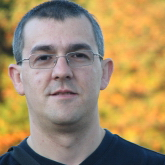
\includegraphics[width=6cm]{content/figures/danny.jpg}
	\end{center}
\end{figure}
\end{frame}

\begin{frame}{Colaboratori}
\begin{figure}[h!]
	\begin{center}
		
\includegraphics[width=6cm]{content/figures/cosmin.jpg}
	\end{center}
\end{figure}
\end{frame}

\begin{frame}{Colaboratori}
\begin{figure}[h!]
	\begin{center}
		
\includegraphics[width=6cm]{content/figures/caius.jpg}
	\end{center}
\end{figure}
\end{frame}

\Large

\section{Introducere}
\begin{frame}{Motiva'tia}
\huge
\begin{itemize}
  \item Trebuie s'a refactoriz'am pentru paralelism
\end{itemize}
\end{frame}

\begin{frame}{Refactorizare}
\Large
Dezavantajele:
\begin{itemize}
  \item \pause transform'arile necesare sunt non-triviale
  \item \pause putem introduce errori 'in foarte multe feluri
\end{itemize}
\end{frame}

\begin{frame}{Refactorizare}
\huge
\textbf{O solu'tie:}
\begin{itemize}
  \item \pause automatizarea refactoriz'arilor
\end{itemize}
\end{frame}

\begin{frame}{ReLooper}
\huge
\begin{itemize}
  \item este un utilitar care paralelizeaza cicluri
  \item \pause nu poate refactoriza dac'a exist'a condi'tii de curs'a
\end{itemize}

\end{frame}

\begin{frame}{Contributia acestei lucrari}
\huge
\begin{itemize}
  \item Corectarea automat'a a condi'tiilor de curs'a
\end{itemize}
\end{frame}

\section{Analiza proiectelor open-source}
\begin{frame}{Analiza proiectelor open-source}
\Huge
\center{34 proiecte}
\normalsize
\pause \begin{itemize}
  \item Jmol
  \item Art of Illusion
  \item Vassal
\end{itemize}
\end{frame}

\begin{frame}
\Huge 
\begin{center}
Ce am g'asit?
\end{center}
\end{frame}

\begin{frame}{Preconditie}
\Huge
\begin{center}Nu putem repara condi'tii de curs'a care au 
dependin'te 'intre itera'tiile ciclului
\end{center}
\pause 
\end{frame}

\begin{frame}[fragile]{Loop carried dependency}
\begin{lstlisting}
//called from within the loop
public void parallelContext() {
    //notice how the field "LCD" is first read
    int temp = this.LCD;
    //...
    this.LCD = 42;
    //...
}
\end{lstlisting}
\end{frame}

\begin{frame}[fragile]{Loop carried dependency}
\begin{lstlisting}
//called from within the loop
public void parallelContext() {
   if(this.condition)
       /*...*/
   else
       this.LCD = 42;    
   
   this.temp = this.LCD
}
\end{lstlisting}
\end{frame}

\begin{frame}{Evaluarea}
\Huge
\begin{itemize}
  \item Jmol, 225 kLoC
\end{itemize}
\end{frame}

\begin{frame}{Evaluare - Loop carried dependency}
\Huge
\begin{itemize}
  \item greu de detectat manual 
  \begin{itemize}
    \item \pause 'in cazuri reale apar 'in cod foarte complex
    \item \pause foarte multe accese la date care trebuiesc inspectate
  \end{itemize} 
\end{itemize}
\end{frame}


\begin{frame}{Rezultate - Loop carried dependencies}
\Large
\begin{itemize}
  \item algoritm \textbf{nou} de determinare a acestora
  \item \pause bazat pe \textit{Interprocedural, Finite,
  Distributive, Subset problem} \textsc{[Reps, Horwitz, Sagiv 1995]}
  \item \pause eficient, timp de rulare de aproximativ 10s 'in cazul Jmol
\end{itemize}
\end{frame}

\begin{frame}{Rezultate - Loop carried dependencies}
\huge
\begin{itemize}
  \item \textbf{163} conditii de cursa
  \item \pause \textbf{63} au fost determinate a fi loop carried dependencies
\end{itemize}
\end{frame}

\begin{frame}[fragile]{Metoda de refactorizare}
\normalsize
\begin{lstlisting}
public class SticksRenderer extends ShapeRenderer {
  private Atom atomA;
  private Atom atomB;
  private Bond bond;
}
\end{lstlisting}

\begin{lstlisting}
public class SticksRenderer extends ShapeRenderer {
  private ThreadLocal<Atom> atomA = 
       new ThreadLocal<Atom>(); 
  private ThreadLocal<Atom> atomB = 
       new ThreadLocal<Atom>();
  private ThreadLocal<Bond> bond = 
       new ThreadLocal<Bond>();
}
\end{lstlisting}
\end{frame}

\begin{frame}{Privatizare}
\Huge
privatizarea datelor
\end{frame}

\begin{frame}{ThreadLocal}
\Large
Dezavantajele \emph{ThreadLocal}-ului:
\begin{itemize}
  \item \pause m'are'ste timpul de execu'tie. 
  \item \pause 'in cazul programului Jmol
  \begin{itemize}
	\Large
    \item \pause \textbf{101} c'ampuri convertite la ThreadLocal
    \item \pause \textbf{997} referiri la aceste c'ampuri
    \item \pause \pause \textbf{63\%} timp 'in plus.
  \end{itemize}
\end{itemize}
\end{frame}

\begin{frame}
\huge
\textbf{{Solutia:}}
\begin{itemize}
  \item \pause privatiz'am la un nivel 'inalt
\end{itemize}
\end{frame}

% \begin{frame}{Preconditie}
% \Huge
% \begin{center}Datele nu au voie s'a aib'a dependin'te 'intre
% itera'tiile ciclului
% \end{center}
% \pause 
% \end{frame}
% 
% \begin{frame}[fragile]{Loop carried dependency}
% \normal
% \begin{lstlisting}
% public void parallelContext() {
%     //notice how the field "LCD" is first read
%     int temp = this.LCD;
%     //...
%     this.LCD = 42;
%     //...
% }
% \end{lstlisting}
% \end{frame}
% 
% \begin{frame}[fragile]{Loop carried dependency}
% \normal
% \begin{lstlisting}
% public void parallelContext() {
%    if(this.condition)
%        /*...*/
%    else
%        this.LCD = 42;    
%    
%    this.temp = this.LCD
% }
% \end{lstlisting}
% \end{frame}
% 
% \begin{frame}{Loop carried dependency}
% \Huge
% \begin{itemize}
%   \item greu de detectat manual 
%   \begin{itemize}
%     \item \pause 'in cazuri reale apar 'in cod foarte complex 
%   \end{itemize} 
% \end{itemize}
% \end{frame}

\begin{frame}{Rezultate - Privatizarea}
\Large
\begin{itemize}
  \item oferim solu'tii pentru privatizare
  \item \pause 20\% din cazuri cea mai eficient'a metod'a de privatizare
  \item \pause restul cazurilor sunt tratate ineficient
\end{itemize}
\end{frame}

\begin{frame}{Rezultate - Refactorizarea}
\begin{itemize}
  \item invocat manual refactorizarea pe 10 c'ampuri reprezentative ale Jmol
  \item \pause a dat rezultatele a'steptate 
\end{itemize}
\end{frame}

\begin{frame}{Contribu'tii}
\begin{itemize}
  \item studiat problema refactoriz'arii pentru paralelism
  \item \pause am implementat un algoritm nou pentru determinearea a loop
  carried dependencies
  \item \pause propus o solutie generic'a pentru rezolvarea condi'tiilor de
  curs'a
  \item \pause propus refactorizarea prin privatizarea datelor
  \item \pause implementat refactorizarile de ThreadLocal si ThreadPrivate
   
%   \item \TODO{studiat problema refac pt paralelism, algoritm pt LCD,
%   identificat tipare de refactorizare si am facut refactorizare prin }
%   \item \TODO{propus o solutie noua}
%   \item \TODO{determinat un algoritm nou}
%   \item \TODO{am propus o varianta threadprivate fata}
%   \item \TODO{refactorizarea prin privatizarea datelor}
%   \item \TODO{am identificat si implementat 10 tipare de rafactorizare}
  
\end{itemize}
\end{frame}


\end{document}
